\newpage
\section{Interfejs użytkownika}
Poniżej znajduje się instrukcja wykonania konkretnych akcji za pomocą interfejsu użytkownika. W pierwszej kolejności zostaną przedstawione akcje, które dostępne są dla mieszkańców.
\subsection{Rejestracja}
Aby się zarejestrować należy wejść na stronę internetową administracji, następnie po wejściu ukazuje się ekran umożliwiający rejestrację lub logowanie. W pierwszej kolejności należy zaznaczyć suwak "Zarejestruj się" (czerwona strzałka), następnie wpisać swoje dane. Kolejną czynnością jest wybranie właściwej nazwy spółdzielni z listy rozwijalnej (strzałka pomarańczowa). Całą czynność należy potwierdzić kliknięciem przycisku "Zarejestruj się" (strzałka czarna).
\begin{figure}[H]
    \centering
    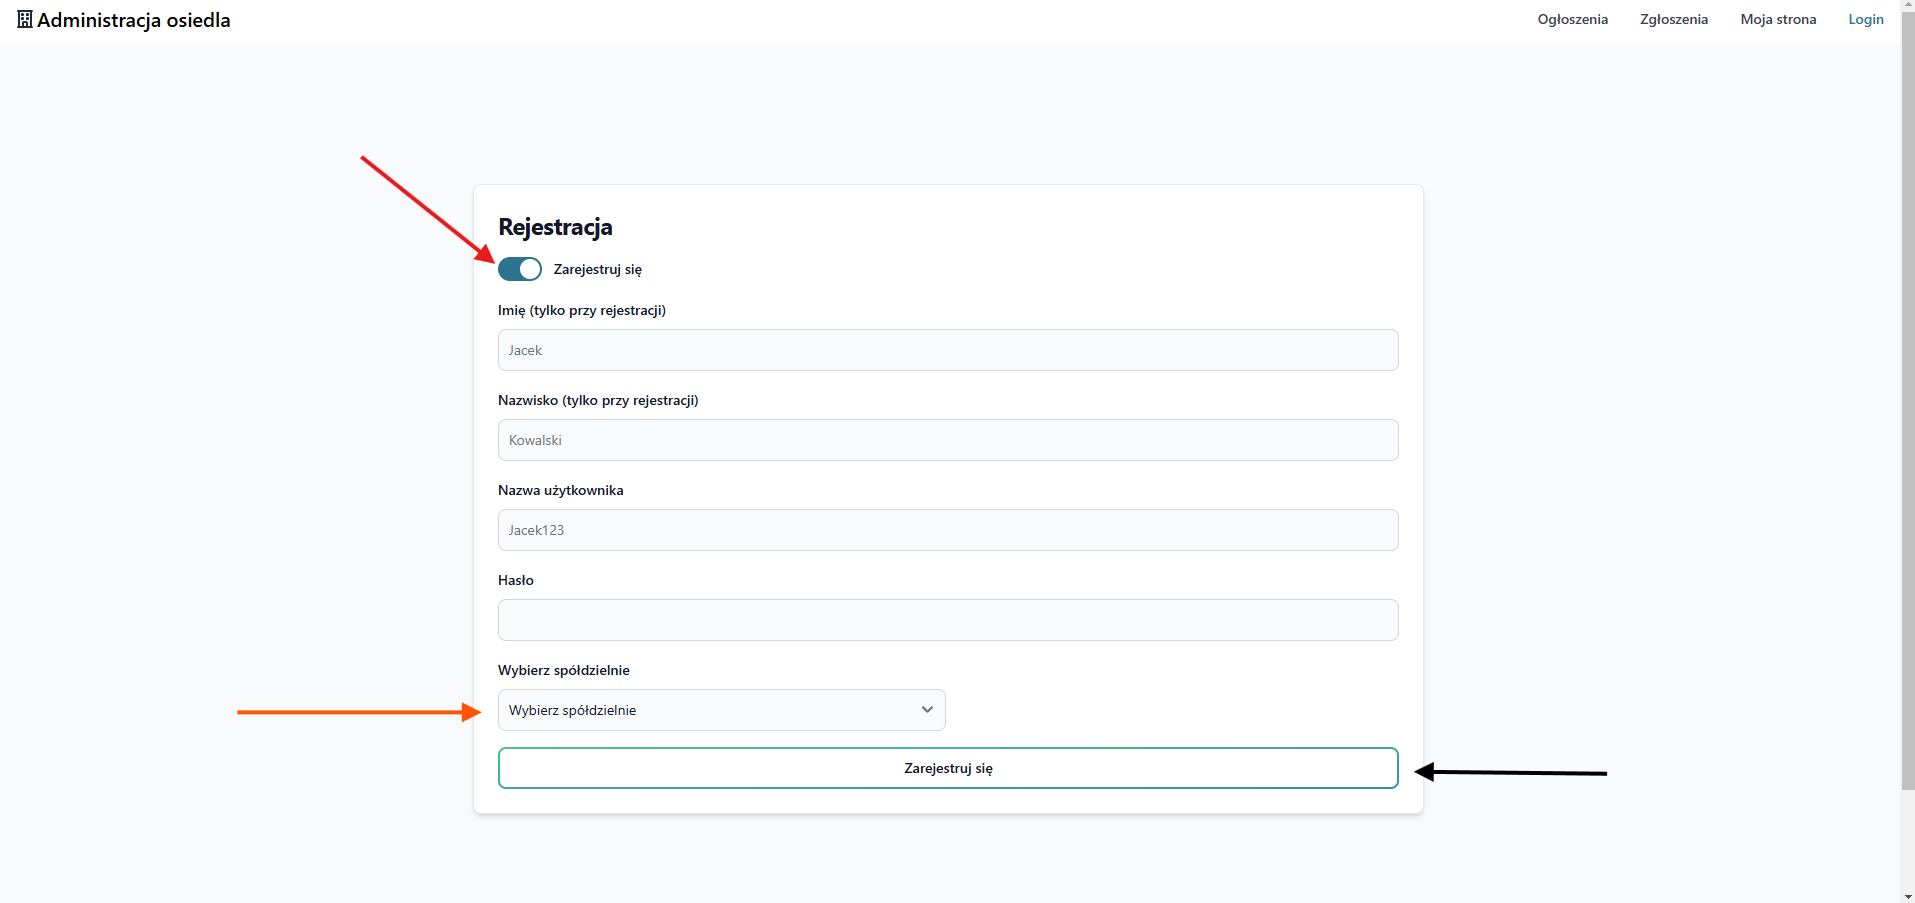
\includegraphics[width=1\linewidth]{img/rejestracja_instrukcja.png}
    \caption{Widok rejestracji}
    \label{fig:register-instr}
\end{figure}
Po poprawnej rejestracji użytkownik zostanie przeniesiony na stronę "Zgłoszenia" a operacja zostanie potwierdzona powiadomieniem "Zarejestrowano pomyślnie" wyświetlającym się w prawym górnym rogu.
\begin{figure}[H]
    \centering
    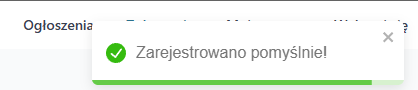
\includegraphics[width=0.75\linewidth]{img/register-succ-toast.png}
    \caption{Widok pomyślnej rejestracji - powiadomienie}
    \label{fig:enter-label}
\end{figure}
\subsection{Logowanie}
Jeśli użytkownik nie jest zalogowany zostanie on przeniesiony na stronę rejestracji/logowania. Aby się zalogować należy wpisać swoją nazwę użytkownika, hasło oraz nacisnąć "Zaloguj się".
\begin{figure}[H]
    \centering
    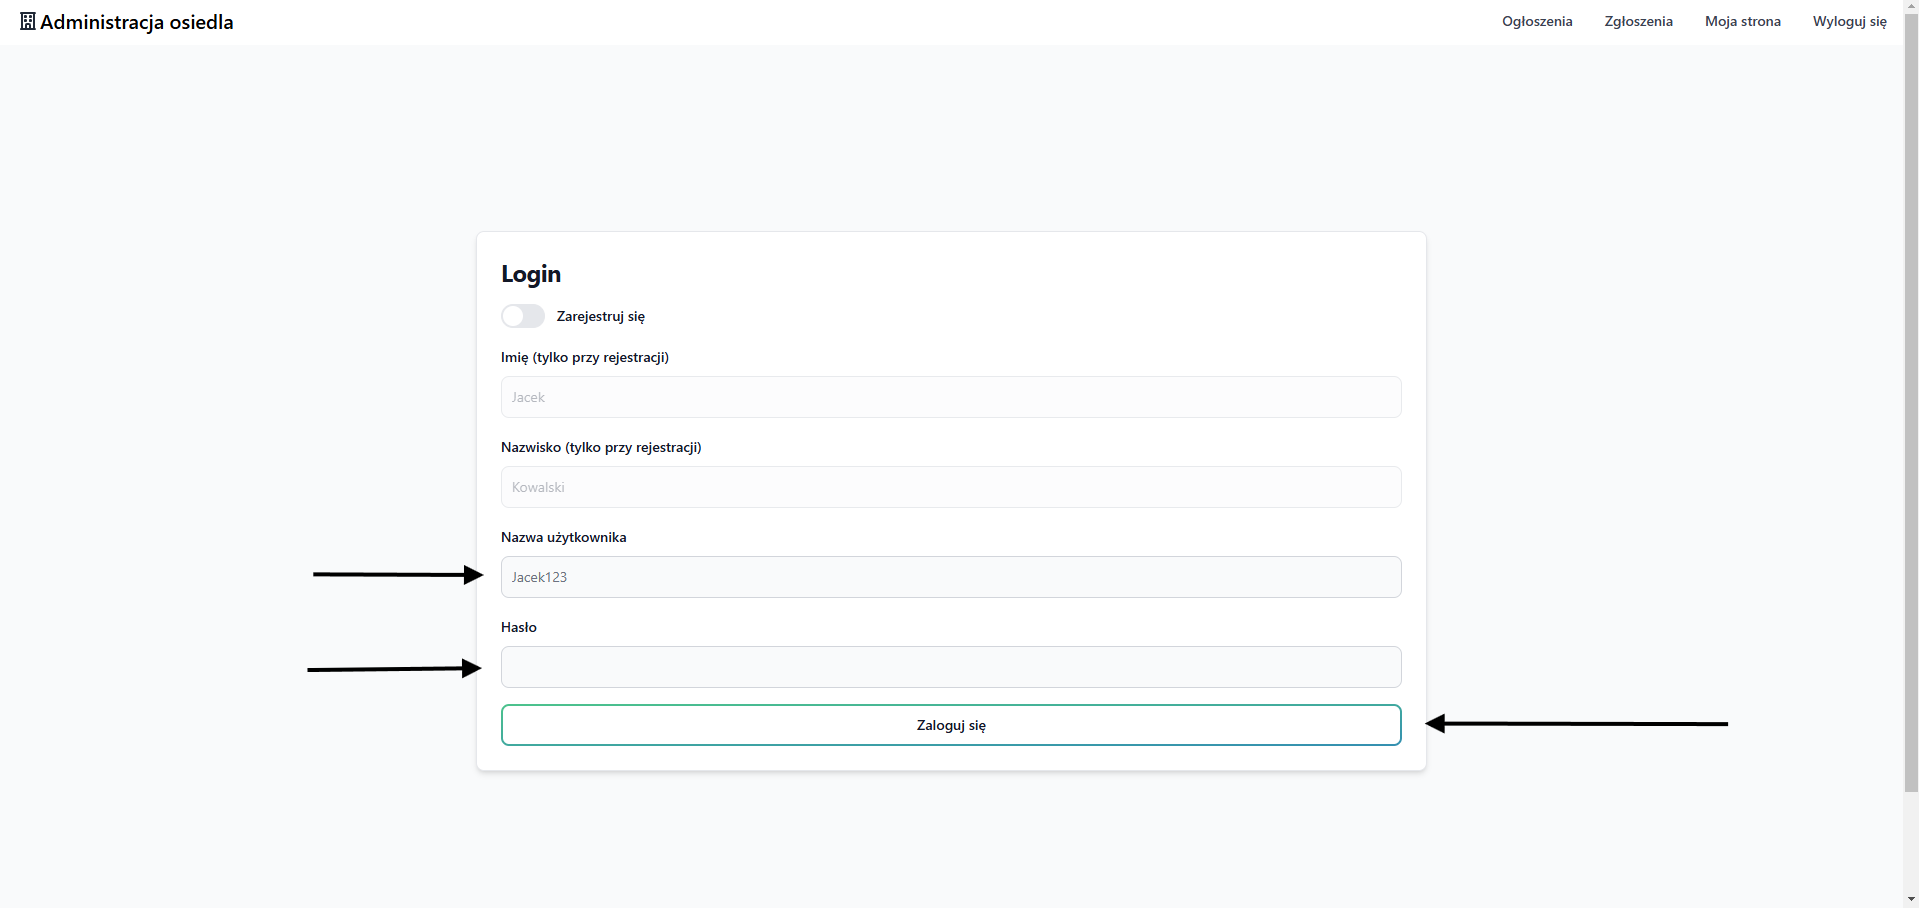
\includegraphics[width=1\linewidth]{img/instruction_login.png}
    \caption{Widok logowania}
    \label{fig:login_instruction}
\end{figure}
Po poprawnej rejestracji użytkownik zostanie przeniesiony na stronę "Zgłoszenia".
\subsection{Wylogowanie}
Aby się wylogować należy nacisnąć przycisk "Wyloguj się".
\begin{figure}[H]
    \centering
    
\includegraphics[width=0.75\linewidth]{img/logout_button.png}
    \caption{Widok wylogowania}
    \label{fig:logout_button}
\end{figure}
Po poprawnym wylogowaniu pokaże się na górze komunikat, a użytkownik zostanie przeniesiony na stronę logowania/rejestracji.
\subsection{Obsługa ogłoszeń}
Aby móc wykonywać operacje związane ze zgłoszeniami należy przejść na stronę "Ogłoszenia" klikając na nią na pasku nawigacji w prawym górnym rogu.
\begin{figure}[H]
    \centering
    
\includegraphics[width=0.75\linewidth]{img/navi_posts.png}
    \caption{Widok paska nawigacji ogłoszeń}
    \label{fig:navi-posts}
\end{figure}
\subsubsection{Dodanie ogłoszenia}
W celu dodania ogłoszenia należy nacisnąć przycisk "Dodaj ogłoszenie".
\begin{figure}[H]
    \centering
    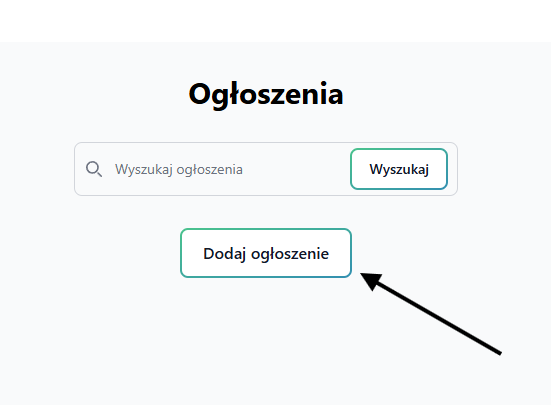
\includegraphics[width=0.75\linewidth]{img/add_post_button2.png}
    \caption{Widok dodania ogłoszenia}
    \label{fig:add-post}
\end{figure}
Następnie należy wypełnić informację o ogłoszeniu: tytuł oraz treść oraz zatwierdzić naciskając "Dodaj ogłoszenie".
\begin{figure}[H]
    \centering
    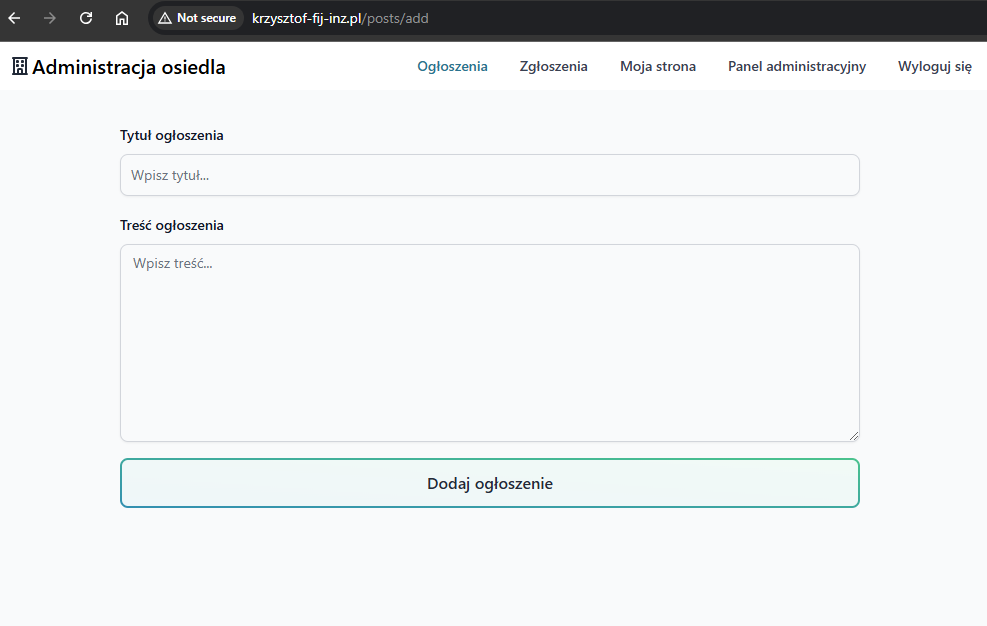
\includegraphics[width=0.75\linewidth]{img/post_add.png}
    \caption{Widok zapisania dodanie ogłoszenia}
    \label{fig:post-add}
\end{figure}
Po poprawnym dodaniu ogłoszenia wyświetli się powiadomienie w prawym górnym rogu potwierdzające dodanie.
\subsubsection{Przeglądanie ogłoszeń}
Wszystkie ogłoszenia naszej spółdzielni znajdują się na stronie ogłoszenia, aby wyszukać ogłoszenie zawierające jakiś tekst należy wpisać ten tekst w pole wyszukiwania i kliknąć wyszukaj.
\begin{figure}[H]
    \centering
    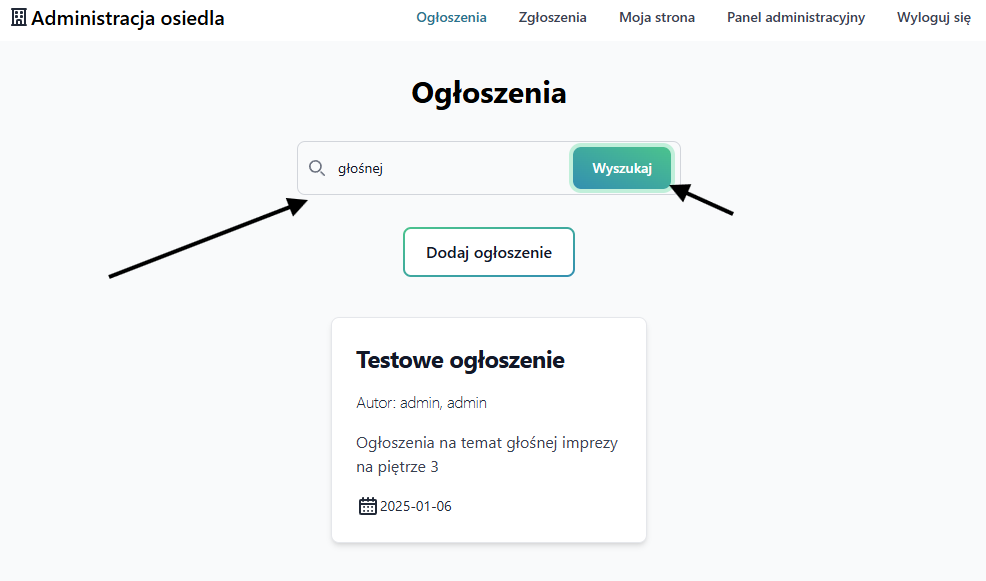
\includegraphics[width=0.75\linewidth]{img/search_posts.png}
    \caption{Widok wyszukania ogłoszeń}
    \label{fig:post-search}
\end{figure}
\subsection{Edytowanie ogłoszeń}
Po kliknięciu w kafelek z ogłoszeniem utworzonym przez nas, widoczny jest przycisk "Edytuj".
\begin{figure}[H]
    \centering
    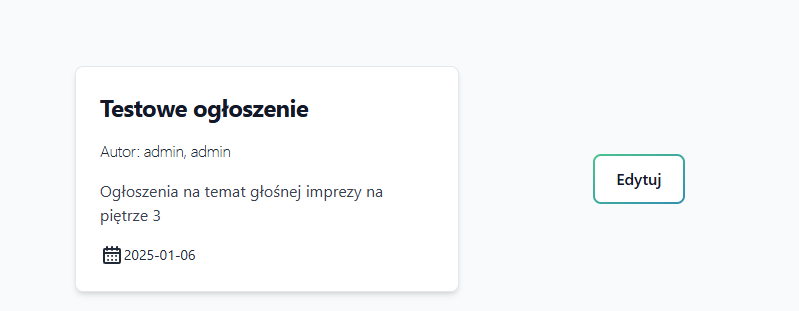
\includegraphics[width=0.75\linewidth]{img/edit_post_button.png}
    \caption{Widok przycisku edycji ogłoszenia}
    \label{fig:edit-post}
\end{figure}
Po naciśnięciu jego jesteśmy w stanie edytować ogłoszenie oraz zapisać edycję, naciskając "Edytuj ogłoszenie".
\begin{figure}[H]
    \centering
    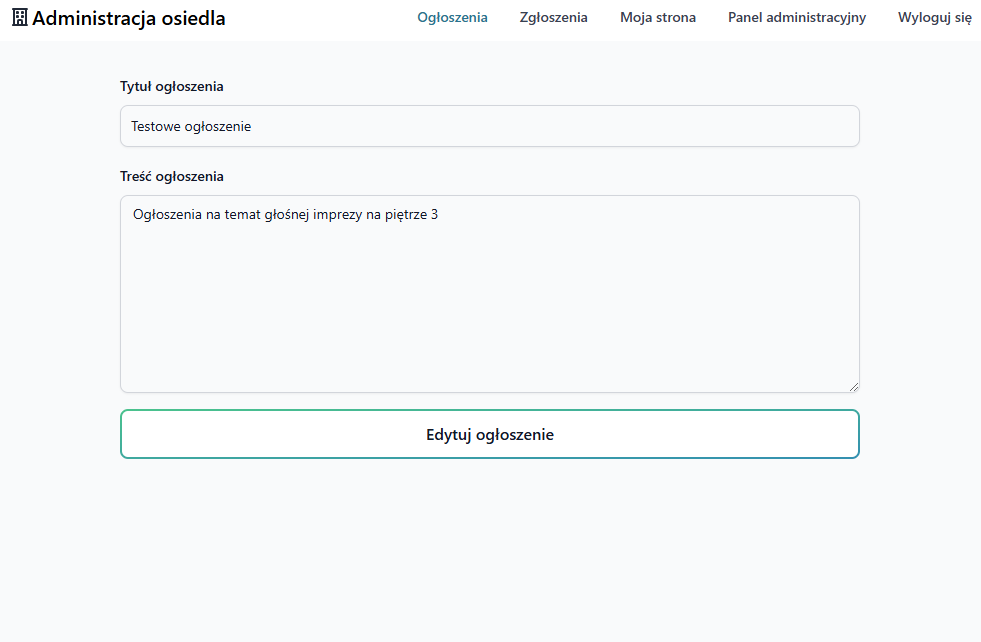
\includegraphics[width=0.75\linewidth]{img/post_edit.png}
    \caption{Widok edycji ogłoszenia}
    \label{fig:edit_post}
\end{figure}
Po naciśnięciu przycisku zapisującego edycję, użytkownik zostaje przeniesiony do strony z ogłoszeniami oraz wyświetlone zostaje powiadomienie potwierdzające edycję ogłoszenia.
\subsection{Moja strona}
Po przejściu na stronę "Moja strona" możemy sprawdzić nasze dane:
\begin{figure}[H]
    \centering
    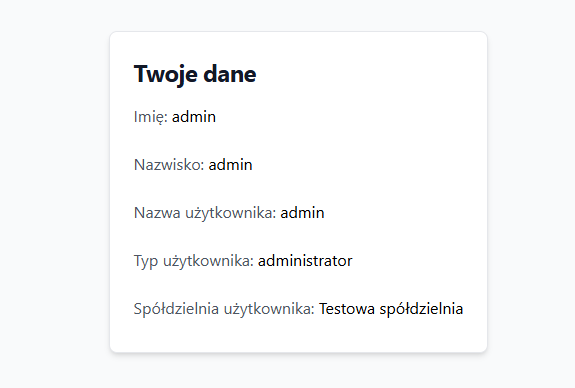
\includegraphics[width=0.75\linewidth]{img/my_page.png}
    \caption{Widok moja strona}
    \label{fig:my_page_view}
\end{figure}
\subsection{Zgłoszenia}
Wyświetlanie, dodawanie i wyszukiwanie zgłoszeń działa analogicznie do ogłoszeń. Zgłoszenia posiadają dodatkową funkcję wyszukiwania naszych zgłoszeń za pomocą przycisku "Moje zgłoszenia".
\begin{figure}[H]
    \centering
    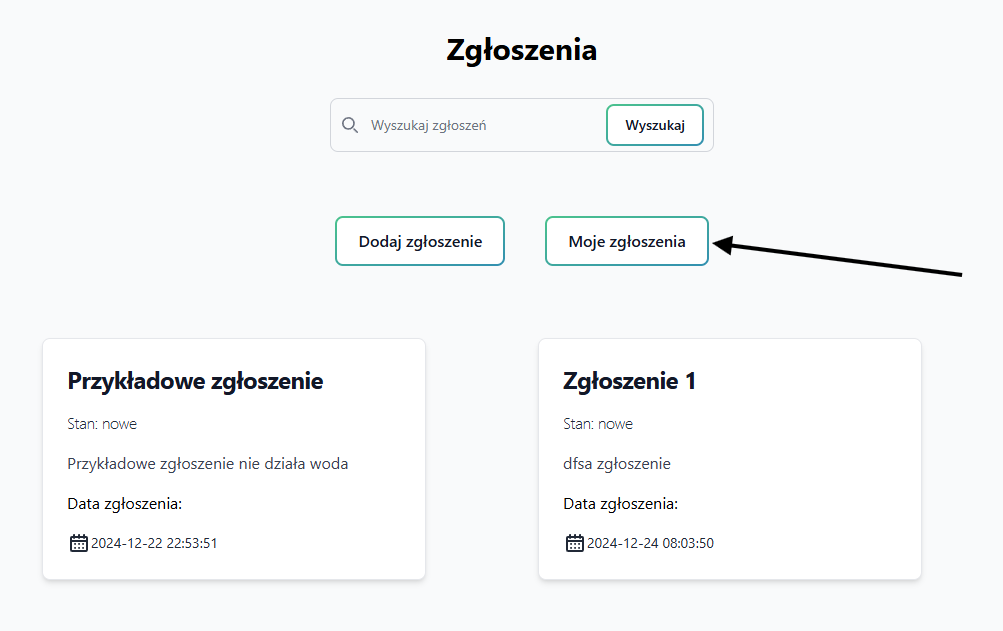
\includegraphics[width=0.75\linewidth]{img/moje_zgloszenia.png}
    \caption{Widok zgłoszeń}
    \label{fig:req-view}
\end{figure}
\subsubsection{Zgłoszenie perspektywa ogólna}
Użytkownik po naciśnięciu na kafelek "Zgłoszenia" wyświetla je oraz może odczytać lub dodać komentarze.
\begin{figure}[H]
    \centering
    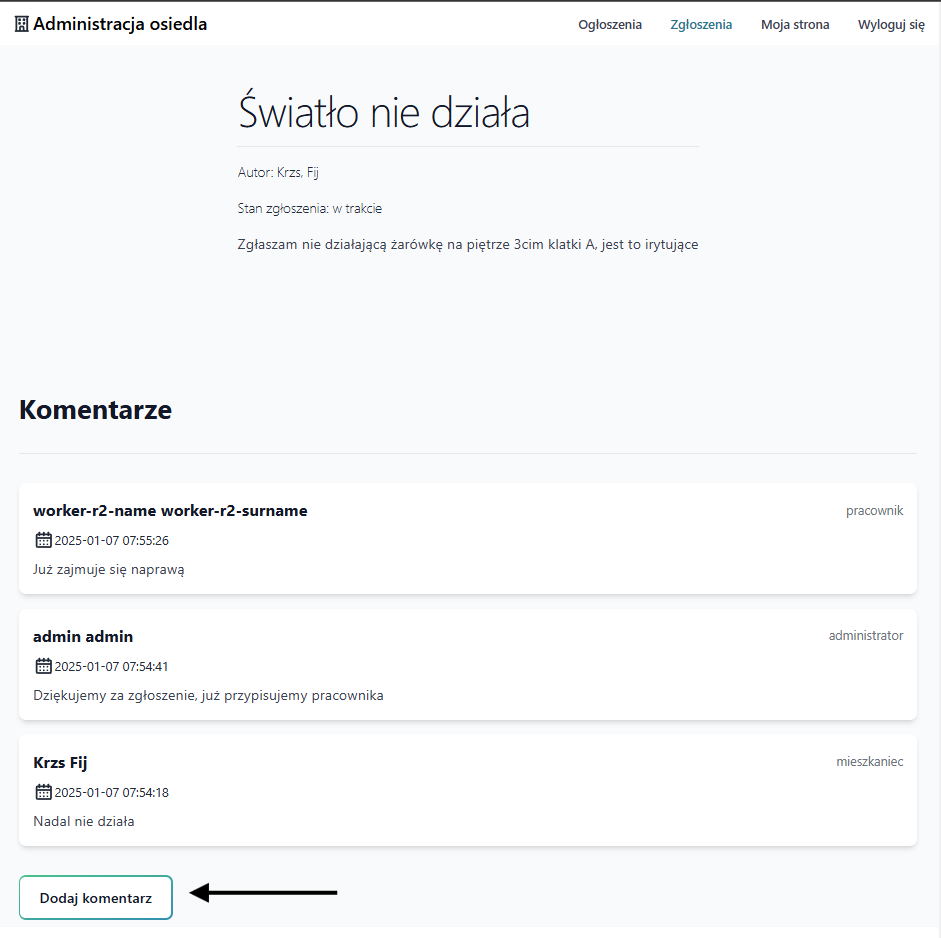
\includegraphics[width=0.75\linewidth]{img/req_user.png}
    \caption{Zgłoszenie widok użytkownika}
    \label{fig:enter-label}
\end{figure}
Aby dodać komentarz, należy nacisnąć przycisk "Dodaj komentarz", po naciśnięciu którego wyświetli się okno z możliwością dodania komentarza, poprawne dodanie zostanie potwierdzone powiadomieniem w prawym górnym rogu.
\begin{figure}[H]
    \centering
    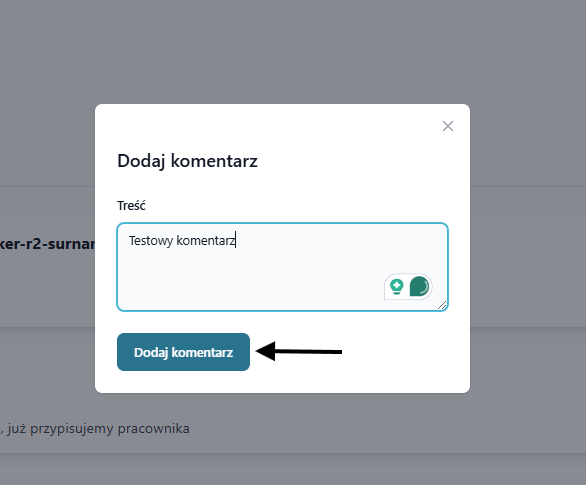
\includegraphics[width=0.5\linewidth]{img/add_comment.png}
    \caption{Widok dodania komentarza}
    \label{fig:add_comment_view}
\end{figure}
\subsubsection{Zgłoszenie perspektywa pracownika}
Pracownik (administrator również jest pracownikiem) może edytować zgłoszenie poprzez przypisanie do niego odpowiedniego działu, widoczności, czy innych parametrów. Zmianę można wykonać poprzez wybranie odpowiednich wartości pól i zapisanie tej zmiany klikając "Zapisz zmiany" (strzałka czarna).
\begin{figure}[H]
    \centering
    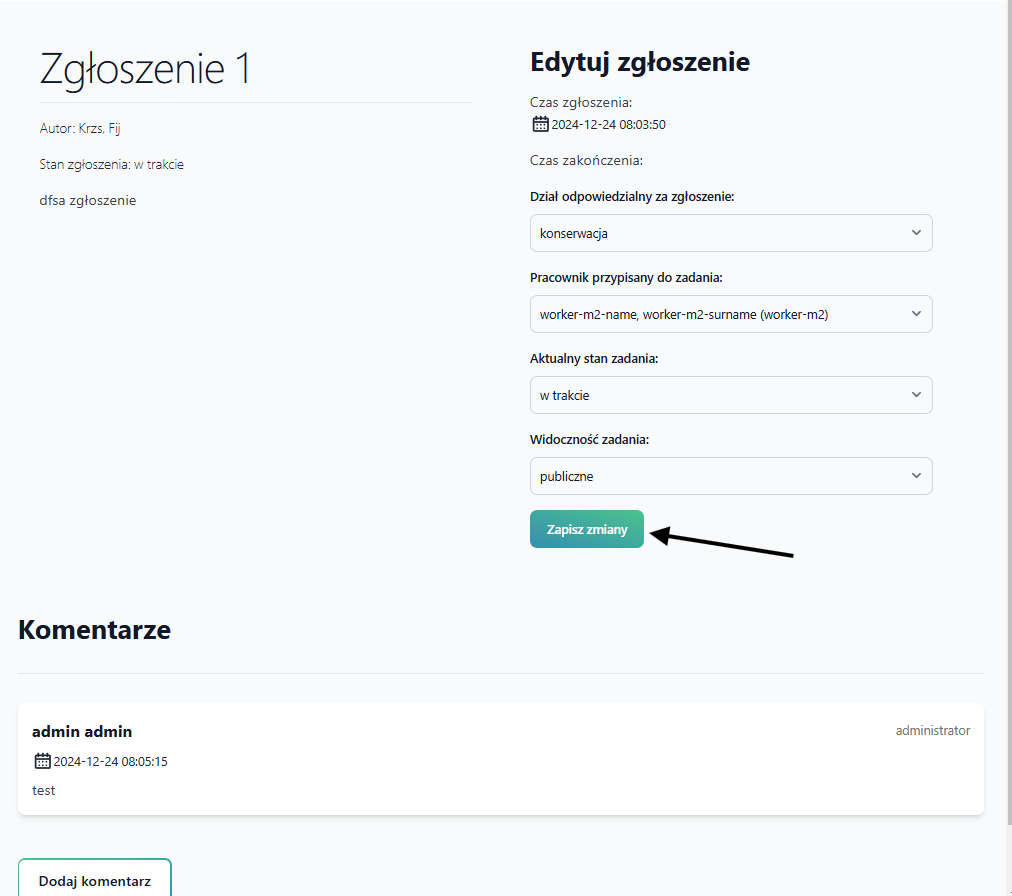
\includegraphics[width=0.75\linewidth]{img/request_worker.png}
    \caption{Zgłoszenie widok pracownika}
    \label{fig:enter-label}
\end{figure}
